\chapter{Directional data}
\label{ch:directional}

Strike and dip, azimuth and elevation, latitude and longitude,
$\ldots$ \textit{directional data} are ubiquitous in the Earth
Sciences. And just like the compositional data discussed in
chapter~\ref{ch:compositional}, the statistical analysis of
directional data is fraught with dangers.

\section{Circular data}
\label{sec:circular}

Consider the following dataset of orientations (in degrees) of thirty
glacial striations from Madagascar:

\begin{center}
\begin{tabular}{ccccccccccccccc}
44 & 51 & 79 & 65 & 27 & 31 & 4 & 355 & 22 & 352 & 287 & 7 & 287 & 339 & 0 \\
276 & 342 & 355 & 334 & 296 & 7 & 17 & 351 & 349 & 37 & 339 & 40 & 324 & 325 & 334\\
\end{tabular}
\end{center}

These values span a range from 0$^{\circ}$ and 360$^{\circ}$, where
$0^{\circ}=360^{\circ}$. Plotting the data on a circle:

\noindent\begin{minipage}[t][][b]{.2\textwidth}
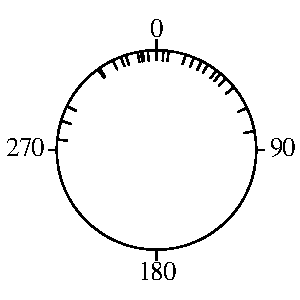
\includegraphics[width=\textwidth]{../figures/circle1.pdf}\\
\end{minipage}
\begin{minipage}[t][][t]{.8\textwidth}
  \captionof{figure}{The orientations of 30~glacial striations. The
    values are roughly centered around zero but exhibit significant
    scatter, from the northwest (276$^\circ$) to the northeast
    (79$^\circ$).\\}
  \label{fig:circle1}
\end{minipage}

Computing the arithmetic mean value of these angles yields a value of
189.2$^{\circ}$. This is a nonsensical value:

\noindent\begin{minipage}[t][][b]{.2\textwidth}
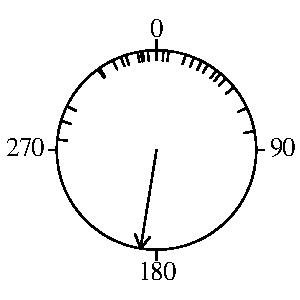
\includegraphics[width=\textwidth]{../figures/circle2.pdf}\\
\end{minipage}
\begin{minipage}[t][][t]{.8\textwidth}
  \captionof{figure}{The same glacial striation data of
    Figure~\ref{fig:circle1}, with their arithmetic mean shown as an
    arrow. Even though the individual striations are all pointing
    north, their arithmetic mean is pointing in exactly the opposite
    direction.\\}
  \label{fig:circle2}
\end{minipage}

The problem is that directional data are `wrapped around' a circle.
The difference between $1^{\circ}$ and $359^{\circ}$ is not
$358^{\circ}$ but $2^{\circ}$. So the usual rules of arithmetic do not
apply to angular measurements. Better results for the difference
between two angles $\theta$ and $\phi$ are obtained using the
following trigonometric relationship:

\begin{equation}
  \theta - \phi = \arcsin\left( \sin[\theta] \cos[\phi] -
                                \cos[\theta] \sin[\phi] \right)
  \label{eq:anglediff}
\end{equation}

For the same reason, the (arithmetic) mean of 1$^\circ$ and
359$^\circ$ is 180$^\circ$ but should be 0$^\circ$. A more sensible
definition of the `mean direction' is again obtained using
trigonometry, by taking the \textbf{vector sum} of all the component
directions. For example, let $\theta = \{\theta_1, \ldots, \theta_i,
\ldots \theta_n \}$ be $n$ angles, then the resultant direction is
obtained by summing the horizontal and vertical components of unit
vectors pointing in these directions:

\begin{equation}
  \overline{\theta} = \arctan\left(\frac{\sum_{i=1}^{n}
    \sin[\theta_i]}{\sum_{i=1}^{n}\cos[\theta_i]} \right)
  \label{eq:averagedirection}
\end{equation}

Applying this formula to the glacial striation data:

\noindent\begin{minipage}[t][][b]{.2\textwidth}
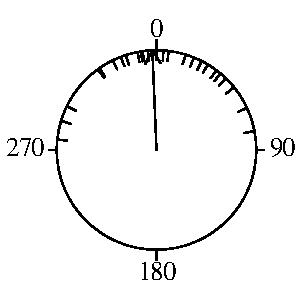
\includegraphics[width=\textwidth]{../figures/circle3.pdf}\\
\end{minipage}
\begin{minipage}[t][][t]{.8\textwidth}
  \captionof{figure}{The direction of the vector sum of the 30 glacial
    striation meausurements points in a direction of 357.6$^\circ$,
    which is marked by the arrow and does a much better job at
    capturing the `central' direction than the arithmetic mean of
    Figure~\ref{fig:circle2} does.\\}
  \label{fig:circle3}
\end{minipage}

Dividing the length of the vector sum by the number of measurements
yields a new summary statistic, $\bar{R}$, which is shown as a thick
black arrow in Figure~\ref{fig:vectorsum}.

\begin{equation}
  \bar{R} = \sqrt{\left(\sum_{i=1}^{n} \sin[\theta_i]/n\right)^2 +
    \left( \sum_{i=1}^{n}\cos[\theta_i]/n \right)^2}
  \label{eq:circularR}
\end{equation}

\noindent\begin{minipage}[t][][b]{.45\textwidth}
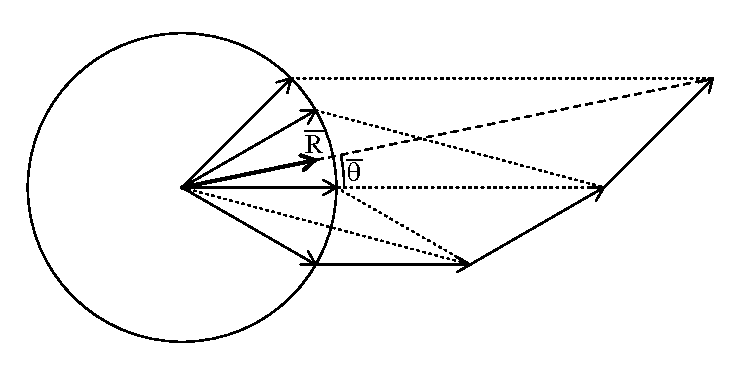
\includegraphics[width=\textwidth]{../figures/vectorsum.pdf}\\
\end{minipage}
\begin{minipage}[t][][t]{.55\textwidth}
  \captionof{figure}{An average direction (dashed line) is obtained by
    taking the vector sum of four angular measurements (thin black
    arrows).  Scaling by the number of measurements (thick black
    arrow) yields a measure of concentration ($0 \leq \bar{R} \leq
    1$), which increases in length with decreasing angular dispersion
    and vice versa.\\}
  \label{fig:vectorsum}
\end{minipage}

This arrow shortens with increasing scatter and so $\bar{R}$ is not
dispersion parameter like the standard deviation, but a
\textit{concentration parameter}. To create a dispersion parameter, we
can use $\bar{R}$ to define the \textbf{circular standard deviation}:

\begin{equation}
  s_c = \sqrt{\ln(1/R^2)}
  \label{eq:circularSD}
\end{equation}

In the extreme case where all the measurements point in the same
direction, $R = 1$ and $s_c = 1$. If the data are evenly distributed
around the circle, $R = 0$ and $s_c = \infty$.

\noindent\begin{minipage}[t][][b]{.2\textwidth}
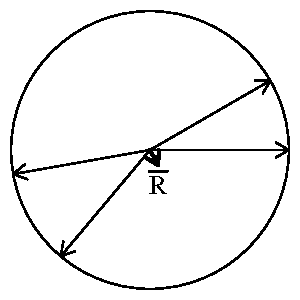
\includegraphics[width=\textwidth]{../figures/lowconcentration.pdf}\\
\end{minipage}
\begin{minipage}[t][][t]{.8\textwidth}
  \captionof{figure}{When the directional measurements are greatly
    dispersed, the normalised vector sum $\bar{R}$ is short
    ($\bar{R}=0.125$ in this example), and the circular standard
    deviation large ($s_c=4.16$).\\}
  \label{fig:lowconcentration}
\end{minipage}

\section{Circular distributions}
\label{sec:circular-distributions}

The normal distribution is not appropriate for directional data for
the same reason why it did not apply to compositional data. Its tails
go from $-\infty$ to $+\infty$ and do not fit within the constrained
dataspace of the angles. The \textbf{von Mises distribution} does not
suffer from this problem:

\begin{equation}
  f(\theta|\mu,\kappa) \propto \exp[\kappa \cos(\theta-\mu)]
  \label{eq:vonMises}
\end{equation}

\noindent where $\mu$ is the location parameter (the mean angle) and
$\kappa$ is the concentration parameter. As the name suggests, large
$\kappa$-values correspond to narrow distributions, and small
$\kappa$-values to wide ones.

\noindent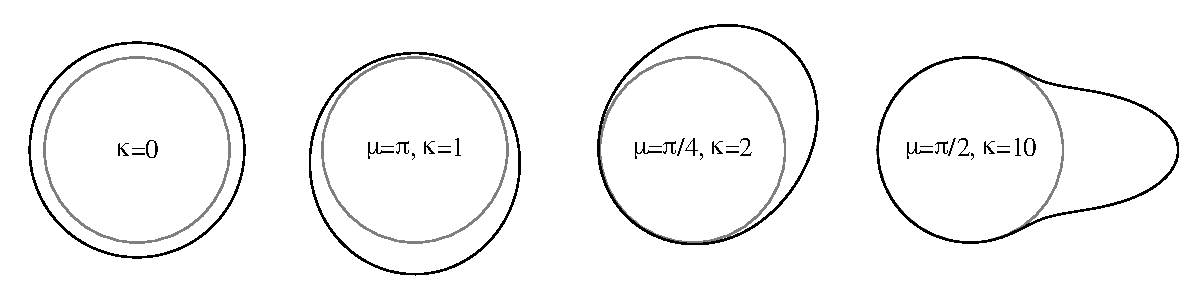
\includegraphics[width=\textwidth]{../figures/vonMises.pdf}
\begingroup \captionof{figure}{Four examples of the von Mises
  distribution with different values for the mean $\mu$ and the
  concentration parameter $\kappa$, wrapped around a (grey)
  circle. The probability density is proportional to the distance
  between this circle and the black line.\\}
\label{fig:vonMises}\endgroup

The parameter $\kappa$ is not easy to determine directly, but can be
estimated indirectly via the concentration parameter $\bar{R}$ and the
following approximation:

\begin{equation}
  \hat{\kappa} = \frac{\bar{R}(p+1-\bar{R}^2)}{1-\bar{R}^2}
  \label{eq:kappa}
\end{equation}

\noindent where $p$ marks the number of parameters, namely $p=1$ for
circular data and $p=2$ for spherical data
(Section~\ref{sec:spherical-distributions}).

\noindent\begin{minipage}[t][][b]{.3\textwidth}
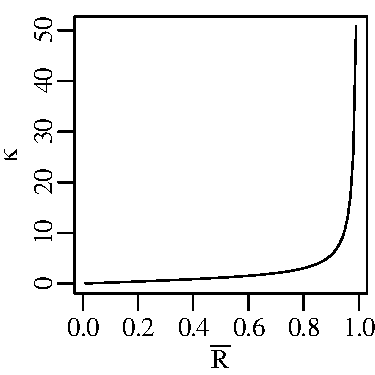
\includegraphics[width=\textwidth]{../figures/R2K.pdf}\\
\end{minipage}
\begin{minipage}[t][][t]{.7\textwidth}
  \captionof{figure}{$\bar{R}$ and $\kappa$ are two concentration
    parameters for circular data. $\bar{R}$ is easier to calculate
    than $\kappa$ (using Equation~\ref{eq:circularR}), and can be
    converted to $\kappa$ in order to fit a von Mises distribution to
    the data.\\}
  \label{fig:R2K}
\end{minipage}

Applying this routine to the glacial striation measurements of
Section~\ref{sec:circular} yields a value of $\bar{R}$ of 0.18, which
corresponds to a $\kappa$-value of 0.37.

\noindent\begin{minipage}[t][][b]{.4\textwidth}
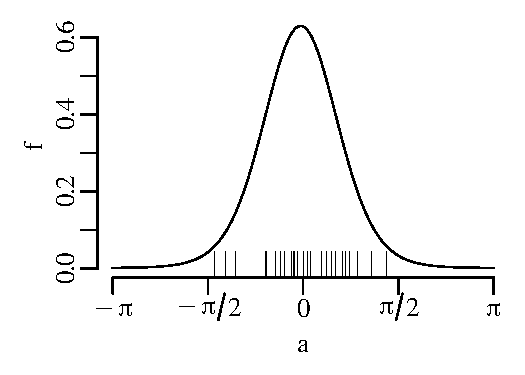
\includegraphics[width=\textwidth]{../figures/kappastriations.pdf}\\
\end{minipage}
\begin{minipage}[t][][t]{.6\textwidth}
  \captionof{figure}{Density plot and rug plot for the glacial
    striation data. The bell shaped density curve represents a von
    Mises distribution with concentration parameter $\kappa=0.37$ and
    mean $\mu=357.6^{\circ}$. In contrast with
    Figure~\ref{fig:vonMises}, in which the von Mises distribution was
    wrapped around a circle, here it is stretched out along a linear
    interval from $-\pi$ to $+\pi$.\\}
  \label{fig:kappastriations}
\end{minipage}

\section{Spherical data}
\label{sec:spherical-data}

The principles of directional statistics can be generalised from the
1-dimensional circular line to a 2-dimensional spherical surface in
3-dimensional space. The coordinates of data in this space can be
expressed as latitude ($l$) and longitude ($L$):

\begin{equation}
  \left\{
  \begin{split}
    x & = \cos[l]\sin[L]\\
    y & = \sin[l]\\
    z & = -\cos[l]\cos[L]
  \end{split}
  \right.
  \label{eq:lL}
\end{equation}

\noindent as strike (S) and dip (D):

\begin{equation}
  \left\{
  \begin{split}
    x & = -\cos[D]\sin[S]\\
    y & = \cos[D]\cos[S]\\
    z & = \sin[D]
  \end{split}
  \right.
  \label{eq:SD}
\end{equation}

\noindent or as dip (D) and azimuth (A):

\begin{equation}
  \left\{
  \begin{split}
    x & = \cos[D] \cos[A]\\
    y & = \cos[D] \sin[A]\\
    z & = \sin[D]
  \end{split}
  \right.
  \label{eq:AD}
\end{equation}

\noindent where the $x$-axis points towards the north, the $y$-axis
towards the east, and the $z$-axis points downwards.  Spherical data
can be visualised on a 2-dimensional surface by stereographic map
projection, using either a Wulff equal angle or a Schmidt equal area
\textbf{stereonet}:

\noindent\begin{minipage}[t][][b]{.6\textwidth}
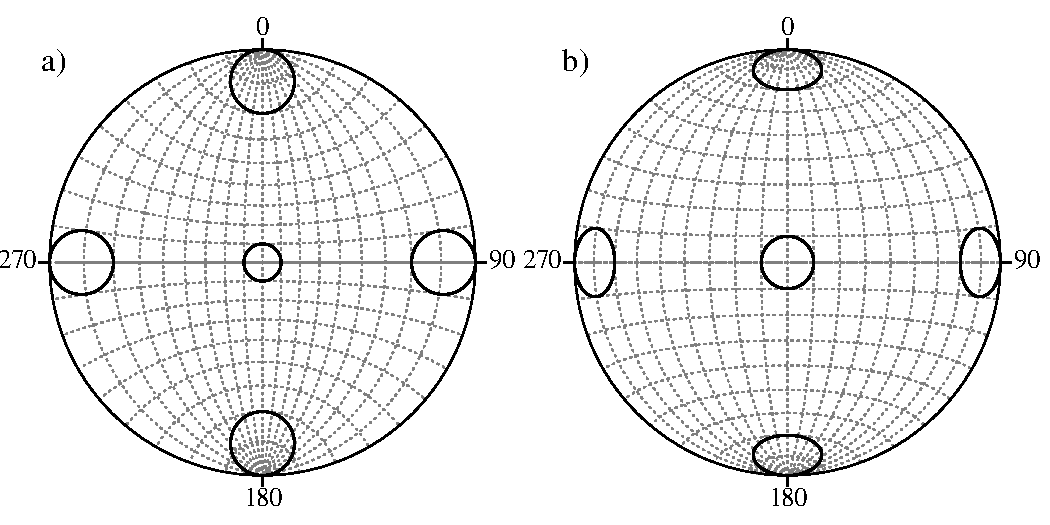
\includegraphics[width=\textwidth]{../figures/wulffschmidt.pdf}\\
\end{minipage}
\begin{minipage}[t][][t]{.4\textwidth}
  \captionof{figure}{a) Wulff equal angle and b) Schmidt equal area
    stereonets, with circles of $10^{\circ}$ radius drawn at azimuths
    of $0^{\circ}, 90^{\circ}, 180^{\circ}$ and $270^{\circ}$, and
    dips of $10^{\circ}$ and $90^\circ$. As the names suggest, the
    Wulff net preserves the shape of the circles, and the Schmidt net
    their area.\\}
  \label{fig:wulffschmidt}
\end{minipage}

The Wulff net is used in structural geology and the Schmidt net in
crystallography. Given the Cartesian coordinates $\{x,y,z\}$, the
stereographic projection proceeds as follows:

\begin{equation}
  \left\{
  \begin{split}
    X & = \tan(\phi) \sin(\theta) \\
    Y & = \tan(\phi) \cos(\theta)
  \end{split}
  \right.
\end{equation}

\noindent for the Wulff net, and 

\begin{equation}
  \left\{
  \begin{split}
    X & = \sqrt{2}\sin(\phi)\sin(\theta) \\
    Y & = \sqrt{2}\sin(\phi)\cos(\theta)
  \end{split}
  \right.
\end{equation}

\noindent for the Schmidt net, where

\begin{equation}
  \left\{
  \begin{split}
    \phi & = \arccos\left(\sqrt{{x^2+y^2+(z-1)^2}}/{2}\right) \\
    \theta & = \arctan\left({x}/{y}\right)
  \end{split}
  \right.
\end{equation}

Stereonets can be used to visualise:

\begin{enumerate}

\item geographical data:

\noindent\begin{minipage}[t][][b]{.6\indentwidth}
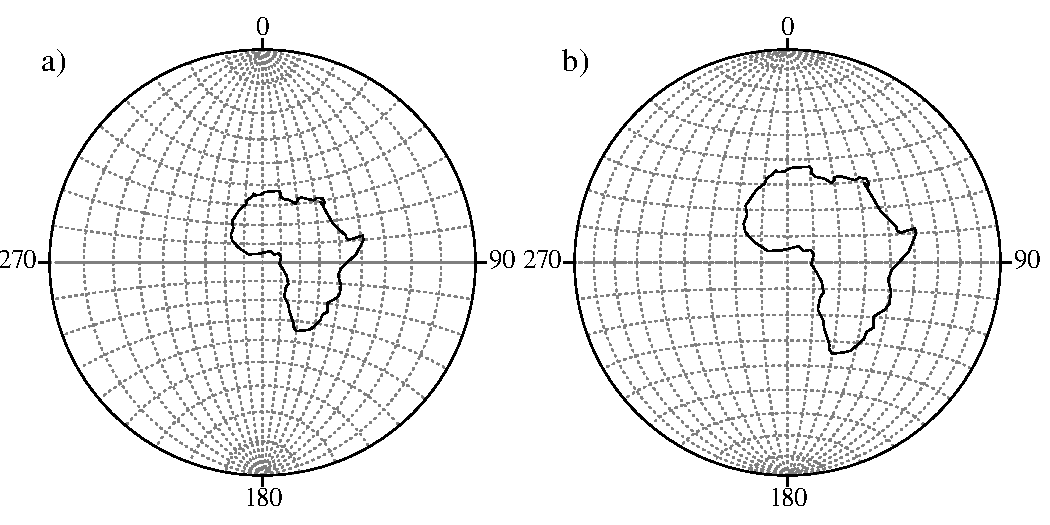
\includegraphics[width=\textwidth]{../figures/Africa.pdf}\\
\end{minipage}
\begin{minipage}[t][][t]{.4\indentwidth}
  \captionof{figure}{a) Wulff and b) Schmidt projection of the African
    continent.  The Wulff net shows Africa in its right shape, the
    Schmidt net shows its right size. No two dimensional projection
    can achieve both goals at once.\\}
  \label{fig:Africa}
\end{minipage}

\item palaeomagnetic data, such as the following dataset of 10
  palaeomagnetic declination (= azimuth) and inclination (= dip)
  measurements:

\begin{tabular}{c|cccccccccc}
declination & 47.9 & 46.3 & 44.7 & 50.9 & 56.4 & 42.6 & 44.9 & 41.5 & 47.9 & 39.6 \\
inclination & 28.6 & 20.1 & 15.6 & 18.1 & 17.5 & 28.7 & 12.2 & 24.5 & 20.6 & 15.0 \\
\end{tabular}

\noindent\begin{minipage}[t][][b]{.3\indentwidth}
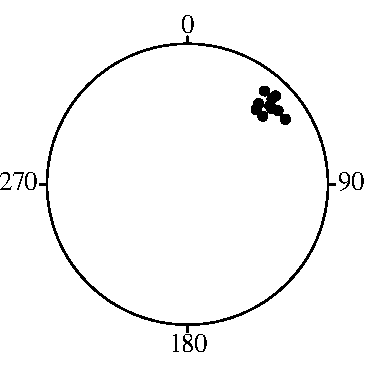
\includegraphics[width=\textwidth]{../figures/palaeomag.pdf}\\
\end{minipage}
\begin{minipage}[t][][t]{.7\indentwidth}
  \captionof{figure}{The palaeomagnetic declination (=azimuth) and
    inclination (=dip) of 10~samples shown in a Schmidt equal area
    diagram.\\}
  \label{fig:palaeomag}
\end{minipage}

\item structural measurements, such as this set of 10 strikes and dips
  on a fault plane:

\begin{tabular}{c|cccccccccc}
strike & 226 & 220 & 223 & 222 & 233 & 227 & 234 & 229 & 227 & 224 \\
dip & 28.4 & 35.3 & 41.0 & 39.6 & 48.3 & 34.7 & 34.5 & 36.0 & 34.2 & 28.7
\end{tabular}  

\noindent\begin{minipage}[t][][b]{.3\indentwidth}
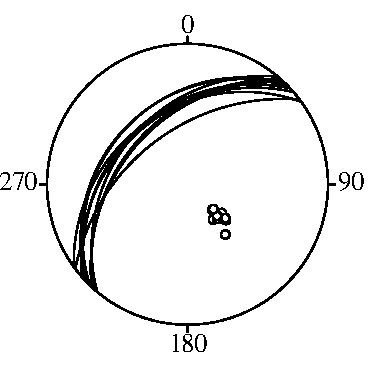
\includegraphics[width=\textwidth]{../figures/fault.pdf}\\
\end{minipage}
\begin{minipage}[t][][t]{.7\indentwidth}
  \captionof{figure}{10 fault plane measurements shown on a Wulff
    stereonet. The white cirles mark the `pole' of the planar
    measurements, i.e. a perpendicular line to the plane. The circular
    segments mark the intersection of the planes with bottom half of a
    sphere, shown in an equal area projection.\\}
  \label{fig:fault}
\end{minipage}

\end{enumerate}

\section{Spherical distributions}
\label{sec:spherical-distributions}

The statistical analysis of spherical data is similar to that of the
circular of Sections~\ref{sec:circular} and
\ref{sec:circular-distributions}. The von Mises -- Fisher (vMF)
distribution generalises the von-Mises distribution of
Equation~\ref{eq:vonMises}.  In three dimensions, the density function
for the vMF distribution is given by:

\begin{equation}
  f(\{x,y,z\}|\{\mu_x,\mu_y,\mu_y\},\kappa) = \frac{\kappa\exp[\kappa
      (x\mu_x+y\mu_y+z\mu_z)]}{2\pi(\exp[\kappa]-\exp[-\kappa])}
  \label{eq:vonMisesFisher}
\end{equation}

\noindent where $\mathbf{\mu}=\{\mu_x,\mu_y,\mu_z\}$ is a unit vector
representing the mean of the distribution in Cartesian coordinates,
and $\kappa$ is the concentration parameter. $\mathbf{\mu}$ and
$\kappa$ are unknown but can be estimated from the data using the
vector sum. To average a collection of $n$ spherical measurements:

\begin{equation}
  \left\{\bar{x},\bar{y},\bar{z}\right\} =
  \left\{\sum_{i=1}^{n}\frac{x_i}{n\bar{R}},
  \sum_{i=1}^{n}\frac{y_i}{n\bar{R}},
  \sum_{i=1}^{n}\frac{z_i}{n\bar{R}}
  \right\}
\end{equation}

\noindent where $\{x_i,y_i,z_i\}$ are the Cartesian coordinates
computed using Equation~\ref{eq:lL}, \ref{eq:SD} or \ref{eq:AD},
and $\bar{R}$ is the concentration parameter:

\begin{equation}
  \bar{R} = \frac{1}{n}
    \sqrt{\left(\sum_{i=1}^{n}x_i\right)^2 +
      \left(\sum_{i=1}^{n}y_i\right)^2 +
      \left(\sum_{i=1}^{n}z_i\right)^2
    }
\end{equation}

\noindent where is related to the (approximate) value for $\kappa$ by
Equation~\ref{eq:kappa} (with $p=2$).

Then the average latitude and longitude are given by:

\begin{equation}
  \left\{
  \begin{split}
  \bar{L} & = \arctan\left(-\bar{x}/\bar{z}\right)\\
  \bar{l} & = \arcsin\left(\bar{y}\right)
  \end{split}
  \right.
\end{equation}

\noindent the average strike and dip:

\begin{equation}
  \left\{
  \begin{split}
    \bar{S} & = \arccos\left(-\bar{x}/\bar{y}\right)\\
    \bar{D} & = \arcsin\left(\bar{z}\right)
  \end{split}
  \right.
\end{equation}

\noindent and the average azimuth and dip:

\begin{equation}
  \left\{
  \begin{split}
    \bar{D} & = \arccos\left(\bar{y}/\bar{x}\right)\\
    \bar{A} & = \arcsin\left(\bar{z}\right)
  \end{split}
  \right.
\end{equation}

Applying this procedure to the palaeomagnetic and structural datasets:

\noindent\begin{minipage}[t][][b]{.6\textwidth}
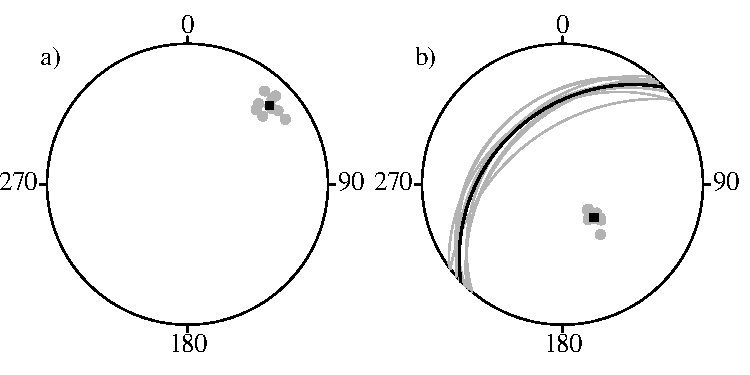
\includegraphics[width=\textwidth]{../figures/sphericalmean.pdf}
\end{minipage}
\begin{minipage}[t][][t]{.4\textwidth}
  \captionof{figure}{a) the palaeomagnetic data of
    Figure~\ref{fig:palaeomag} shown in grey, with their vector mean
    marked as a black square. b) the fault data of
    Figure~\ref{fig:fault} in grey with the vector mean as a back
    square and great circle.\\}
  \label{fig:sphericalmean}
\end{minipage}

